% Fig. 4.10 / CH4_FIGURE_SPECS.md line 4622 -- the two ways of naming the same
%   point: the right-tail point z_alpha, and the left boundary that carries the
%   same area, written both as -z_alpha and as z_{1-alpha}.
% Source: mathstatch4.tex lines 4622-4664 (\label{tailprob}).
%
% Same density as normal-right-tail-point.tex (Fig. 4.5),
%   f(x) = 0.3989423 e^{-x^2/2},  |x| <= 3.5,
% the x unit being one standard deviation, and the same boundary at 1.645,
% where the curve stands 0.1031108 and each tail carries 0.05 of the area.  The
% manuscript draws 3.069 e^{-(x-4)^2/3} and puts its two boundaries at x = 7 and
% x = 1, i.e. +-2.449 standard deviations; per CH2_FIGURE_SPECS.md 1.6 the web
% version uses a genuine density, and the boundary is moved in for the reason
% recorded in Fig. 4.5 (at 2.449 the block is a sliver that closes up at the
% 350px phone width).  No number appears in the picture or in the caption.
%
% The x scale is 1.05cm rather than the 1.08cm of Figs. 4.4 and 4.5: this
% picture carries an alpha outside the curve at each end and the wide label
% -z_alpha = z_{1-alpha}, and at 1.08cm the drawing would be 8.92cm wide, which
% drops the scriptscript type at the 350px phone width to 11.04px, i.e. to the
% 11px floor of spec 1.3 with nothing to spare.  This figure stands on a page of
% its own, so nothing has to be read against it at one scale.
%
% Deviations from the manuscript picture:
%
% 1. The manuscript draws both boundaries as solid black lines.  Here they are
%    journalmuted dashed 0.5pt guides dropping from their points on the curve
%    to the axis, per CH2_FIGURE_SPECS.md 1.6, with a tick mark carrying each
%    position on the axis.  Same treatment as Fig. 4.5.
%
% 2. Colours per spec 1.2: the two blocks are journalaccent at 0.15 rather than
%    grey at 0.2, and the two arrows and the two alphas are journalaccent.
%
% 3. The two curved dashed arrows keep the manuscript's arrangement -- each
%    leaves its block at half the height of the curve there (|x| = 2.3,
%    f = 0.0283, so 0.0141) and bends outward, with alpha written at its head
%    -- but are shortened so that the heads and their labels stay inside the
%    picture.  An invisible \path at the left balances the axis label at the
%    right, so the curve sits centred in the SVG.
%
% Size and type.  Native size measured from the produced SVG:
% 245.802 x 76.57 pt (drawing range 8.53cm wide, inside the 9.0cm cap of
% spec 1.3).  A mark of S pt shows at
% S x 0.99626 x <display width> / 245.802 px, so at the 350px phone width of a
% topic-figure--wide in body text
%     10pt text 14.18px, 8pt scriptscripts 11.35px
% and at the 620px desktop width 25.12 / 20.10px.  The marks at scriptscript
% size are the alpha of z_alpha and the 1-alpha of z_{1-alpha}, which \sssig
% sets there as the manuscript does; \DeclareMathSizes{10}{10}{9}{8} raises
% them from the default 5pt, per spec 1.3.  Checked in the SVG: those alphas
% have 3.5781pt of ink against 4.4844pt for the alphas at text size, i.e.
% 0.798, the 8/10 the declaration asks for and not the 0.5 of the default.
\documentclass[tikz,border=2pt]{standalone}
\usepackage{amsmath}
\usepackage{amssymb}
\usepackage{xcolor}
\usetikzlibrary{arrows.meta}
\newcommand{\sssig}{\scriptscriptstyle}
\DeclareMathSizes{10}{10}{9}{8}

\definecolor{journalink}{HTML}{1F1C18}
\definecolor{journalmuted}{HTML}{8A7F72}
\definecolor{journalaccent}{HTML}{9C2D2D}

% standard normal density, argument in standard deviations
\newcommand{\normaldensity}[1]{0.3989423*exp(-(#1)*(#1)/2)}

\begin{document}
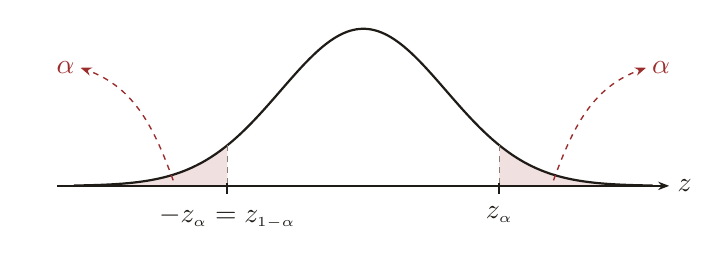
\begin{tikzpicture}[
  x=1.05cm,
  y=5cm,
  every node/.style={font=\normalsize, journalink},
  axis/.style={journalink, line width=0.8pt, -{Stealth[length=4pt]}},
  tick/.style={journalink, line width=0.8pt},
  curve/.style={journalink, line width=0.8pt},
  guide/.style={journalmuted, line width=0.5pt, dash pattern=on 2pt off 2pt},
  region/.style={journalaccent, fill opacity=0.15},
  pointer/.style={journalaccent, line width=0.5pt,
                  dash pattern=on 2pt off 2pt, -{Stealth[length=4pt]}}
]
  % ---- left edge, set against the axis label at the right --------------
  \path (-4.06,0);

  % ---- the two tail blocks ---------------------------------------------
  \fill[region]
    (1.645,0) -- (3.5,0) -- (3.5,0.0008727)
    -- plot[domain=3.5:1.645, samples=300, smooth] (\x,{\normaldensity{\x}})
    -- cycle;
  \fill[region]
    (-3.5,0) -- (-1.645,0) -- (-1.645,0.1031108)
    -- plot[domain=-1.645:-3.5, samples=300, smooth] (\x,{\normaldensity{\x}})
    -- cycle;

  % ---- density curve ---------------------------------------------------
  \draw[curve] plot[domain=-3.5:3.5, samples=300, smooth]
    (\x,{\normaldensity{\x}});

  % ---- the two boundaries ----------------------------------------------
  \draw[guide] ( 1.645,0.1031108) -- ( 1.645,0);
  \draw[guide] (-1.645,0.1031108) -- (-1.645,0);
  \draw[tick] ([yshift=0.035cm] 1.645,0) -- ([yshift=-0.106cm] 1.645,0);
  \draw[tick] ([yshift=0.035cm]-1.645,0) -- ([yshift=-0.106cm]-1.645,0);
  \node[anchor=north, inner sep=0pt] at ([yshift=-0.25cm]1.645,0)
    {$z_{\sssig \alpha}$};
  \node[anchor=north, inner sep=0pt] at ([yshift=-0.25cm]-1.645,0)
    {$-z_{\sssig \alpha} = z_{\sssig 1-\alpha}$};

  % ---- x axis ----------------------------------------------------------
  \draw[axis] (-3.7,0) -- (3.7,0);
  \node[anchor=west, inner sep=2.8pt] at (3.7,0) {$z$};

  % ---- the area of each block, named at the head of its arrow ----------
  \draw[pointer] ( 2.3,0.0141) to[out= 70, in= 200] ( 3.42,0.30);
  \draw[pointer] (-2.3,0.0141) to[out=110, in=-20] (-3.42,0.30);
  \node[journalaccent, anchor=west, inner sep=2pt] at ( 3.42,0.30) {$\alpha$};
  \node[journalaccent, anchor=east, inner sep=2pt] at (-3.42,0.30) {$\alpha$};

\end{tikzpicture}
\end{document}
